\documentclass[tikz, border=10pt]{standalone}
\usepackage{tikz}
\usepackage{amsmath}
\usetikzlibrary{shapes, calc, backgrounds, arrows.meta}

\begin{document}
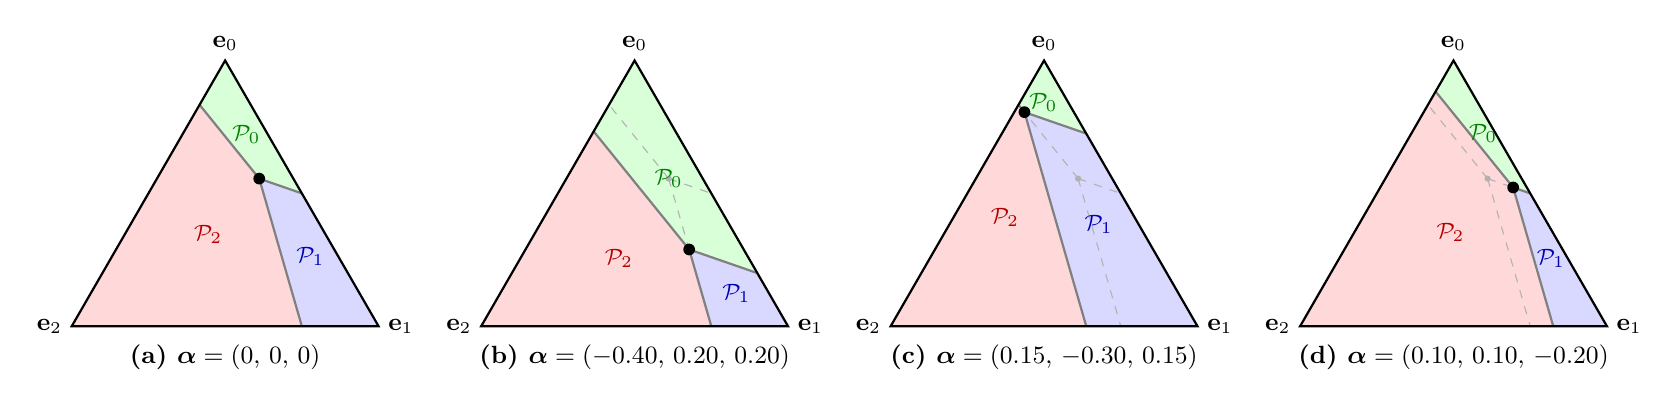
\begin{tikzpicture}[font=\sffamily]

    \begin{scope}[xshift=0.0cm, scale=0.45]
    \coordinate (Top) at (0.000, 5.000);
    \coordinate (Right) at (4.330, -2.500);
    \coordinate (Left) at (-4.330, -2.500);

    \coordinate (Int) at (0.962, 1.667);

    \fill[green!15] (0.000, 5.000) -- (2.165, 1.250) -- (0.962, 1.667) -- (-0.722, 3.750) -- cycle;
    \fill[blue!15] (4.330, -2.500) -- (2.165, -2.500) -- (0.962, 1.667) -- (2.165, 1.250) -- cycle;
    \fill[red!15] (-4.330, -2.500) -- (-0.722, 3.750) -- (0.962, 1.667) -- (2.165, -2.500) -- cycle;

    \draw[thick, black!50] (Int) -- (2.165, 1.250);
    \draw[thick, black!50] (Int) -- (-0.722, 3.750);
    \draw[thick, black!50] (Int) -- (2.165, -2.500);

    \draw[thick] (Top) -- (Right) -- (Left) -- cycle;

    \node[circle, fill=black, inner sep=1.5pt] at (Int) {};

    \node[green!50!black, font=\footnotesize\bfseries] at (0.601, 2.917) {$\mathcal{P}_0$};
    \node[blue!70!black, font=\footnotesize\bfseries] at (2.406, -0.521) {$\mathcal{P}_1$};
    \node[red!70!black, font=\footnotesize\bfseries] at (-0.481, 0.104) {$\mathcal{P}_2$};

    \node[above, font=\small] at (Top) {$\mathbf{e}_0$};
    \node[right, font=\small] at (Right) {$\mathbf{e}_1$};
    \node[left, font=\small] at (Left) {$\mathbf{e}_2$};
    \node[font=\small\bfseries, anchor=north, align=center] at (0, -2.750) {(a) $\boldsymbol{\alpha} = (0,\,0,\,0)$};
    \end{scope}

    \begin{scope}[xshift=5.2cm, scale=0.45]
    \coordinate (Top) at (0.000, 5.000);
    \coordinate (Right) at (4.330, -2.500);
    \coordinate (Left) at (-4.330, -2.500);

    \coordinate (Int) at (1.540, -0.333);

    \fill[green!15] (0.000, 5.000) -- (3.464, -1.000) -- (1.540, -0.333) -- (-1.155, 3.000) -- cycle;
    \fill[blue!15] (4.330, -2.500) -- (2.165, -2.500) -- (1.540, -0.333) -- (3.464, -1.000) -- cycle;
    \fill[red!15] (-4.330, -2.500) -- (-1.155, 3.000) -- (1.540, -0.333) -- (2.165, -2.500) -- cycle;

    \coordinate (OvInt) at (0.962, 1.667);
    \draw[dashed, gray!60, thin] (OvInt) -- (2.165, 1.250);
    \draw[dashed, gray!60, thin] (OvInt) -- (-0.722, 3.750);
    \draw[dashed, gray!60, thin] (OvInt) -- (2.165, -2.500);
    \node[circle, fill=gray!60, inner sep=0.8pt] at (OvInt) {};

    \draw[thick, black!50] (Int) -- (3.464, -1.000);
    \draw[thick, black!50] (Int) -- (-1.155, 3.000);
    \draw[thick, black!50] (Int) -- (2.165, -2.500);

    \draw[thick] (Top) -- (Right) -- (Left) -- cycle;

    \node[circle, fill=black, inner sep=1.5pt] at (Int) {};

    \node[green!50!black, font=\footnotesize\bfseries] at (0.962, 1.667) {$\mathcal{P}_0$};
    \node[blue!70!black, font=\footnotesize\bfseries] at (2.875, -1.583) {$\mathcal{P}_1$};
    \node[red!70!black, font=\footnotesize\bfseries] at (-0.445, -0.583) {$\mathcal{P}_2$};

    \node[above, font=\small] at (Top) {$\mathbf{e}_0$};
    \node[right, font=\small] at (Right) {$\mathbf{e}_1$};
    \node[left, font=\small] at (Left) {$\mathbf{e}_2$};
    \node[font=\small\bfseries, anchor=north, align=center] at (0, -2.750) {(b) $\boldsymbol{\alpha} = (-0.40,\,0.20,\,0.20)$};
    \end{scope}

    \begin{scope}[xshift=10.4cm, scale=0.45]
    \coordinate (Top) at (0.000, 5.000);
    \coordinate (Right) at (4.330, -2.500);
    \coordinate (Left) at (-4.330, -2.500);

    \coordinate (Int) at (-0.553, 3.542);

    \fill[green!15] (0.000, 5.000) -- (1.191, 2.938) -- (-0.553, 3.542) -- (-0.722, 3.750) -- cycle;
    \fill[blue!15] (4.330, -2.500) -- (1.191, -2.500) -- (-0.553, 3.542) -- (1.191, 2.938) -- cycle;
    \fill[red!15] (-4.330, -2.500) -- (-0.722, 3.750) -- (-0.553, 3.542) -- (1.191, -2.500) -- cycle;

    \coordinate (OvInt) at (0.962, 1.667);
    \draw[dashed, gray!60, thin] (OvInt) -- (2.165, 1.250);
    \draw[dashed, gray!60, thin] (OvInt) -- (-0.722, 3.750);
    \draw[dashed, gray!60, thin] (OvInt) -- (2.165, -2.500);
    \node[circle, fill=gray!60, inner sep=0.8pt] at (OvInt) {};

    \draw[thick, black!50] (Int) -- (1.191, 2.938);
    \draw[thick, black!50] (Int) -- (-0.722, 3.750);
    \draw[thick, black!50] (Int) -- (1.191, -2.500);

    \draw[thick] (Top) -- (Right) -- (Left) -- cycle;

    \node[circle, fill=black, inner sep=1.5pt] at (Int) {};

    \node[green!50!black, font=\footnotesize\bfseries] at (-0.021, 3.807) {$\mathcal{P}_0$};
    \node[blue!70!black, font=\footnotesize\bfseries] at (1.540, 0.370) {$\mathcal{P}_1$};
    \node[red!70!black, font=\footnotesize\bfseries] at (-1.104, 0.573) {$\mathcal{P}_2$};

    \node[above, font=\small] at (Top) {$\mathbf{e}_0$};
    \node[right, font=\small] at (Right) {$\mathbf{e}_1$};
    \node[left, font=\small] at (Left) {$\mathbf{e}_2$};
    \node[font=\small\bfseries, anchor=north, align=center] at (0, -2.750) {(c) $\boldsymbol{\alpha} = (0.15,\,-0.30,\,0.15)$};
    \end{scope}

    \begin{scope}[xshift=15.600000000000001cm, scale=0.45]
    \coordinate (Top) at (0.000, 5.000);
    \coordinate (Right) at (4.330, -2.500);
    \coordinate (Left) at (-4.330, -2.500);

    \coordinate (Int) at (1.684, 1.417);

    \fill[green!15] (0.000, 5.000) -- (2.165, 1.250) -- (1.684, 1.417) -- (-0.505, 4.125) -- cycle;
    \fill[blue!15] (4.330, -2.500) -- (2.815, -2.500) -- (1.684, 1.417) -- (2.165, 1.250) -- cycle;
    \fill[red!15] (-4.330, -2.500) -- (-0.505, 4.125) -- (1.684, 1.417) -- (2.815, -2.500) -- cycle;

    \coordinate (OvInt) at (0.962, 1.667);
    \draw[dashed, gray!60, thin] (OvInt) -- (2.165, 1.250);
    \draw[dashed, gray!60, thin] (OvInt) -- (-0.722, 3.750);
    \draw[dashed, gray!60, thin] (OvInt) -- (2.165, -2.500);
    \node[circle, fill=gray!60, inner sep=0.8pt] at (OvInt) {};

    \draw[thick, black!50] (Int) -- (2.165, 1.250);
    \draw[thick, black!50] (Int) -- (-0.505, 4.125);
    \draw[thick, black!50] (Int) -- (2.815, -2.500);

    \draw[thick] (Top) -- (Right) -- (Left) -- cycle;

    \node[circle, fill=black, inner sep=1.5pt] at (Int) {};

    \node[green!50!black, font=\footnotesize\bfseries] at (0.836, 2.948) {$\mathcal{P}_0$};
    \node[blue!70!black, font=\footnotesize\bfseries] at (2.748, -0.583) {$\mathcal{P}_1$};
    \node[red!70!black, font=\footnotesize\bfseries] at (-0.084, 0.135) {$\mathcal{P}_2$};

    \node[above, font=\small] at (Top) {$\mathbf{e}_0$};
    \node[right, font=\small] at (Right) {$\mathbf{e}_1$};
    \node[left, font=\small] at (Left) {$\mathbf{e}_2$};
    \node[font=\small\bfseries, anchor=north, align=center] at (0, -2.750) {(d) $\boldsymbol{\alpha} = (0.10,\,0.10,\,-0.20)$};
    \end{scope}

\end{tikzpicture}
\end{document}
